\documentclass[12pt,a4paper]{article}

% ── Packages ──────────────────────────────────────────────────────────────────
\usepackage[T1]{fontenc}
\usepackage[utf8]{inputenc}
\usepackage[margin=2.5cm]{geometry}
\usepackage{lmodern}
\usepackage{microtype}
\usepackage{parskip}
\usepackage{titlesec}
\usepackage{enumitem}
\usepackage{booktabs}
\usepackage{xcolor}
\usepackage{hyperref}
\usepackage{listings}
\usepackage{tikz}
\usetikzlibrary{shapes,arrows,positioning,fit,backgrounds}

% ── Colour palette ────────────────────────────────────────────────────────────
\definecolor{mpblue}{HTML}{1A73E8}
\definecolor{mpgreen}{HTML}{34A853}
\definecolor{mporange}{HTML}{EA8600}
\definecolor{mpgray}{HTML}{5F6368}
\definecolor{codebg}{HTML}{F8F9FA}
\definecolor{codeframe}{HTML}{DADCE0}

% ── Hyperref setup ────────────────────────────────────────────────────────────
\hypersetup{
    colorlinks=true,
    linkcolor=mpblue,
    urlcolor=mpblue,
    citecolor=mpblue,
    pdftitle={MediaPipe Tutorial 01 -- Getting Started},
    pdfauthor={MediaPipe Tutorials},
}

% ── Listings (code blocks) ────────────────────────────────────────────────────
\lstdefinestyle{pythonstyle}{
    language=Python,
    backgroundcolor=\color{codebg},
    frame=single,
    framerule=0.8pt,
    rulecolor=\color{codeframe},
    basicstyle=\ttfamily\small,
    keywordstyle=\color{mpblue}\bfseries,
    stringstyle=\color{mpgreen},
    commentstyle=\color{mpgray}\itshape,
    numberstyle=\tiny\color{mpgray},
    numbers=left,
    numbersep=8pt,
    breaklines=true,
    breakatwhitespace=true,
    showstringspaces=false,
    tabsize=4,
    captionpos=b,
}
\lstset{style=pythonstyle}

\lstdefinestyle{bashstyle}{
    language=bash,
    backgroundcolor=\color{codebg},
    frame=single,
    framerule=0.8pt,
    rulecolor=\color{codeframe},
    basicstyle=\ttfamily\small,
    keywordstyle=\color{mporange}\bfseries,
    commentstyle=\color{mpgray}\itshape,
    breaklines=true,
    showstringspaces=false,
}

% ── Section formatting ────────────────────────────────────────────────────────
\titleformat{\section}{\large\bfseries\color{mpblue}}{}{0em}{}[\titlerule]
\titleformat{\subsection}{\normalsize\bfseries\color{mpgray}}{}{0em}{}

% ── TikZ styles ───────────────────────────────────────────────────────────────
\tikzset{
    block/.style={
        rectangle, rounded corners=4pt,
        draw=mpblue, fill=mpblue!10,
        text width=2.8cm, align=center,
        minimum height=1.2cm,
        font=\small\bfseries
    },
    sideblock/.style={
        rectangle, rounded corners=4pt,
        draw=mporange, fill=mporange!10,
        text width=5cm, align=center,
        minimum height=0.9cm,
        font=\small
    },
    arrow/.style={->, >=stealth, thick, color=mpblue},
    sidearrow/.style={->, >=stealth, dashed, color=mporange},
    label/.style={font=\footnotesize\color{mpgray}, align=center},
}

% ─────────────────────────────────────────────────────────────────────────────
\begin{document}

\title{%
    \vspace{-1cm}
    \textbf{\textcolor{mpblue}{MediaPipe Tutorial 01}}\\[0.4em]
    \large Getting Started: Installation, Core Concepts,\\
    and Your First Face-Detection Pipeline
}
\author{MediaPipe Tutorials Series}
\date{\today}
\maketitle

\tableofcontents
\newpage

% ─────────────────────────────────────────────────────────────────────────────
\section{Introduction}

MediaPipe is Google's open-source, cross-platform framework for real-time perception
pipelines. It powers features such as Google Meet background segmentation, Pixel camera
effects, and YouTube AR filters. This tutorial guides you from a fresh Python environment to
a working face-detection demo, while building a solid conceptual foundation for the advanced
tutorials that follow.

% ─────────────────────────────────────────────────────────────────────────────
\section{Installation}

\subsection{Via pip (recommended)}

\begin{lstlisting}[style=bashstyle, caption={Installing MediaPipe via pip}]
# Create a virtual environment
python -m venv mp-env
source mp-env/bin/activate   # Windows: mp-env\Scripts\activate

# Install MediaPipe and dependencies
pip install mediapipe opencv-python numpy
\end{lstlisting}

\subsection{Verify the installation}

\begin{lstlisting}[caption={Verify installation}]
import mediapipe as mp
import cv2
import numpy as np

print("MediaPipe:", mp.__version__)
print("OpenCV   :", cv2.__version__)
print("NumPy    :", np.__version__)
\end{lstlisting}

% ─────────────────────────────────────────────────────────────────────────────
\section{MediaPipe Graph Pipeline --- Architecture Diagram}

The diagram below illustrates the dataflow inside a MediaPipe graph.
Every solution (face detection, hand tracking, pose estimation \ldots) is
realised as such a graph.

\bigskip

\begin{center}
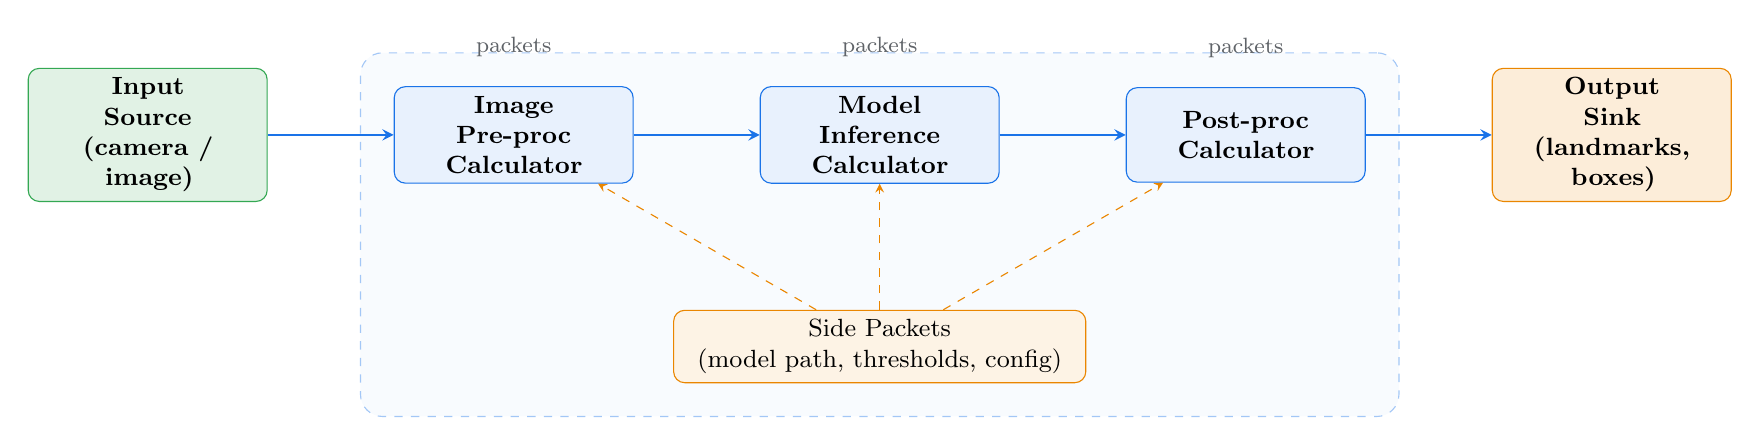
\begin{tikzpicture}[node distance=1.2cm and 1.6cm]

    % Nodes
    \node[block, fill=mpgreen!15, draw=mpgreen] (src)
        {Input\\Source\\(camera /\\image)};

    \node[block, right=of src] (pre)
        {Image\\Pre-proc\\Calculator};

    \node[block, right=of pre] (inf)
        {Model\\Inference\\Calculator};

    \node[block, right=of inf] (post)
        {Post-proc\\Calculator};

    \node[block, fill=mporange!15, draw=mporange, right=of post] (sink)
        {Output\\Sink\\(landmarks,\\boxes)};

    % Side packet node
    \node[sideblock, below=1.6cm of inf] (side)
        {Side Packets\\(model path, thresholds, config)};

    % Arrows (main pipeline)
    \draw[arrow] (src)  -- (pre);
    \draw[arrow] (pre)  -- (inf);
    \draw[arrow] (inf)  -- (post);
    \draw[arrow] (post) -- (sink);

    % Arrows (side packets)
    \draw[sidearrow] (side) -- (pre);
    \draw[sidearrow] (side) -- (inf);
    \draw[sidearrow] (side) -- (post);

    % Background frame
    \begin{scope}[on background layer]
        \node[draw=mpblue!40, dashed, rounded corners=8pt,
              fill=mpblue!3,
              fit=(pre)(inf)(post)(side),
              inner sep=12pt,
              label={[label, anchor=north west]north west:MediaPipe Graph (.pbtxt)}
              ] {};
    \end{scope}

    % Stream labels
    \node[label, above=0.25cm of pre] {packets};
    \node[label, above=0.25cm of inf] {packets};
    \node[label, above=0.25cm of post] {packets};

\end{tikzpicture}
\end{center}

\bigskip

% ─────────────────────────────────────────────────────────────────────────────
\section{Core Concepts}

\subsection{Graphs}

A MediaPipe \textbf{graph} is a Protocol Buffer text file (\texttt{.pbtxt}) that declares
calculators and the typed streams connecting them.

\subsection{Calculators}

A \textbf{calculator} is a C++ class (or Python wrapper) implementing three lifecycle
methods: \texttt{GetContract()} to declare input/output types, \texttt{Open()} for one-time
initialisation, and \texttt{Process()} for per-packet logic.

\subsection{Packets and Streams}

A \textbf{packet} is a timestamped, strongly-typed value.
A \textbf{stream} is an ordered sequence of packets flowing between two calculators.
A \textbf{side packet} is a one-time configuration value injected at graph startup.

% ─────────────────────────────────────────────────────────────────────────────
\section{Solutions API vs Tasks API}

\begin{center}
\begin{tabular}{lll}
\toprule
\textbf{Feature} & \textbf{Solutions API} & \textbf{Tasks API} \\
\midrule
Status & Legacy (still supported) & Current (recommended) \\
Platforms & Python only & Python, Android, iOS, Web \\
Model format & Embedded in package & \texttt{.task} bundle file \\
Live-stream mode & Manual loop & Built-in callback \\
\bottomrule
\end{tabular}
\end{center}

% ─────────────────────────────────────────────────────────────────────────────
\section{Hello-World: Face Detection}

\begin{lstlisting}[caption={Complete face-detection webcam demo}]
"""
Tutorial 01 - Hello-World Face Detection
Uses the MediaPipe Solutions API for simplicity.
"""

import cv2
import mediapipe as mp

mp_face_detection = mp.solutions.face_detection

def draw_detections(frame, detections):
    h, w, _ = frame.shape
    for detection in detections:
        bbox = detection.location_data.relative_bounding_box
        x1 = int(bbox.xmin * w)
        y1 = int(bbox.ymin * h)
        bw = int(bbox.width * w)
        bh = int(bbox.height * h)
        score = detection.score[0]
        cv2.rectangle(frame, (x1, y1), (x1+bw, y1+bh), (0, 255, 0), 2)
        cv2.putText(frame, f"{score:.0%}", (x1, y1-8),
                    cv2.FONT_HERSHEY_SIMPLEX, 0.6, (0, 255, 0), 2)

def main():
    cap = cv2.VideoCapture(0)
    with mp_face_detection.FaceDetection(
        model_selection=0,
        min_detection_confidence=0.5
    ) as detector:
        while True:
            ret, frame = cap.read()
            if not ret:
                break
            rgb = cv2.cvtColor(frame, cv2.COLOR_BGR2RGB)
            rgb.flags.writeable = False
            results = detector.process(rgb)
            rgb.flags.writeable = True
            frame = cv2.cvtColor(rgb, cv2.COLOR_RGB2BGR)
            if results.detections:
                draw_detections(frame, results.detections)
            cv2.imshow("Face Detection", frame)
            if cv2.waitKey(1) & 0xFF == ord('q'):
                break
    cap.release()
    cv2.destroyAllWindows()

if __name__ == "__main__":
    main()
\end{lstlisting}

% ─────────────────────────────────────────────────────────────────────────────
\section{Troubleshooting}

\begin{description}[style=nextline]
    \item[\textcolor{mporange}{Camera permissions (Linux)}]
        \lstinline[style=bashstyle]{sudo usermod -aG video $USER} then log out and back in.
    \item[\textcolor{mporange}{Wrong webcam index}]
        Try \texttt{VideoCapture(1)}, \texttt{(2)}, \ldots{}
        List devices with \lstinline[style=bashstyle]{v4l2-ctl --list-devices}.
    \item[\textcolor{mporange}{Model download fails behind proxy}]
        Set \lstinline[style=bashstyle]{export HTTPS_PROXY=http://proxy:8080}.
    \item[\textcolor{mporange}{Slow frame rate}]
        Set \texttt{rgb.flags.writeable = False}, reduce resolution, or use
        \texttt{model\_selection=0}.
\end{description}

% ─────────────────────────────────────────────────────────────────────────────
\section{Next Steps}

Proceed to Tutorial~02 where you will work with Face Mesh's 478 landmarks,
estimate face distances, and track multiple faces simultaneously.

\end{document}
